\section{Diskussion}
\label{sec:Diskussion}

Die berechneten Spaltbreiten der Einzelspalte werden mit den Herstellerangaben verglichen:
\begin{align*}
  &\text{Spaltbreite:} & b_\text{1,exp} &= (\num{0.1462 +- 0.0035})\,\si{\milli\meter} \\
  &\text{Herstellerangabe:} & b_\text{1,th} &= 0,15\,\si{\milli\meter} \\
  &\text{Abweichung:} & p_1 &= \num{2,53}\,\%.\\ \\
  &\text{Spaltbreite:} & b_\text{2,exp} &= (\num{0.338 +- 0.005}) \,\si{\milli\meter} \\
  &\text{Herstellerangabe:} & b_\text{2,th} &= 0,4\,\si{\milli\meter} \\
  &\text{Abweichung:} & p_2 &= \num{15,50}\,\%.
\end{align*}

Hierbei wird deutlich, dass diese relativ wenig von den Herstellerangaben abweichen.
Es ist jedoch anzumerken, dass für die Ausgleichsrechnungen jeweils Anfangsparameter festgelegt
werden mussten, sodass nicht gewährleistet ist, dass die berechneten Ausgleichsfunktionen
treffend sind. Da diese dem Verlauf der Messwerte jedoch sehr gut folgen, und da
die aus den Parametern der Ausgleichsrechnung berechneten Werte für die Spaltbreiten
relativ nah an den jeweiligen Herstellerangaben liegen, ist jedoch
anzunehmen, dass die Ausgleichsrechnungen recht genau und sinnvoll erfolgt sind.

Auffällig ist, dass die Messwerte selbst nach Bereinigung um den Dunkelstrom nie
den Wert null Annehmen, wie es jedoch theoretisch anzunehmen wäre. Ein möglicher Grund
hierfür ist eine unzureichende Schärfe des Interferenzbildes. Dies ist besonders beim
Doppelspalt zu beobachten.

Bei dem Vergleich zwischen der Beugungsfiguren von Doppel- und Einzelspalt sollte zu
erkennen sein, dass die des Einzelspalts die Einhüllende des Doppelspalts sein soll, wenn die
des Doppelspalts dementsprechend skaliert wurde. Dies ist nicht zu erkennen, was  
daran liegt, dass die zum Doppelspalt gehörige Ausgleichsfunktion 
trotz Angabe der zu den Herstellerangaben passenden
Anfangsparameter nicht richtig erfolgte.


\section{Anhang}
\label{sec:Anhang}
Im folgenden sind die Kopien der Messwerte aufgelistet.
\begin{figure}[H]
  \centering
  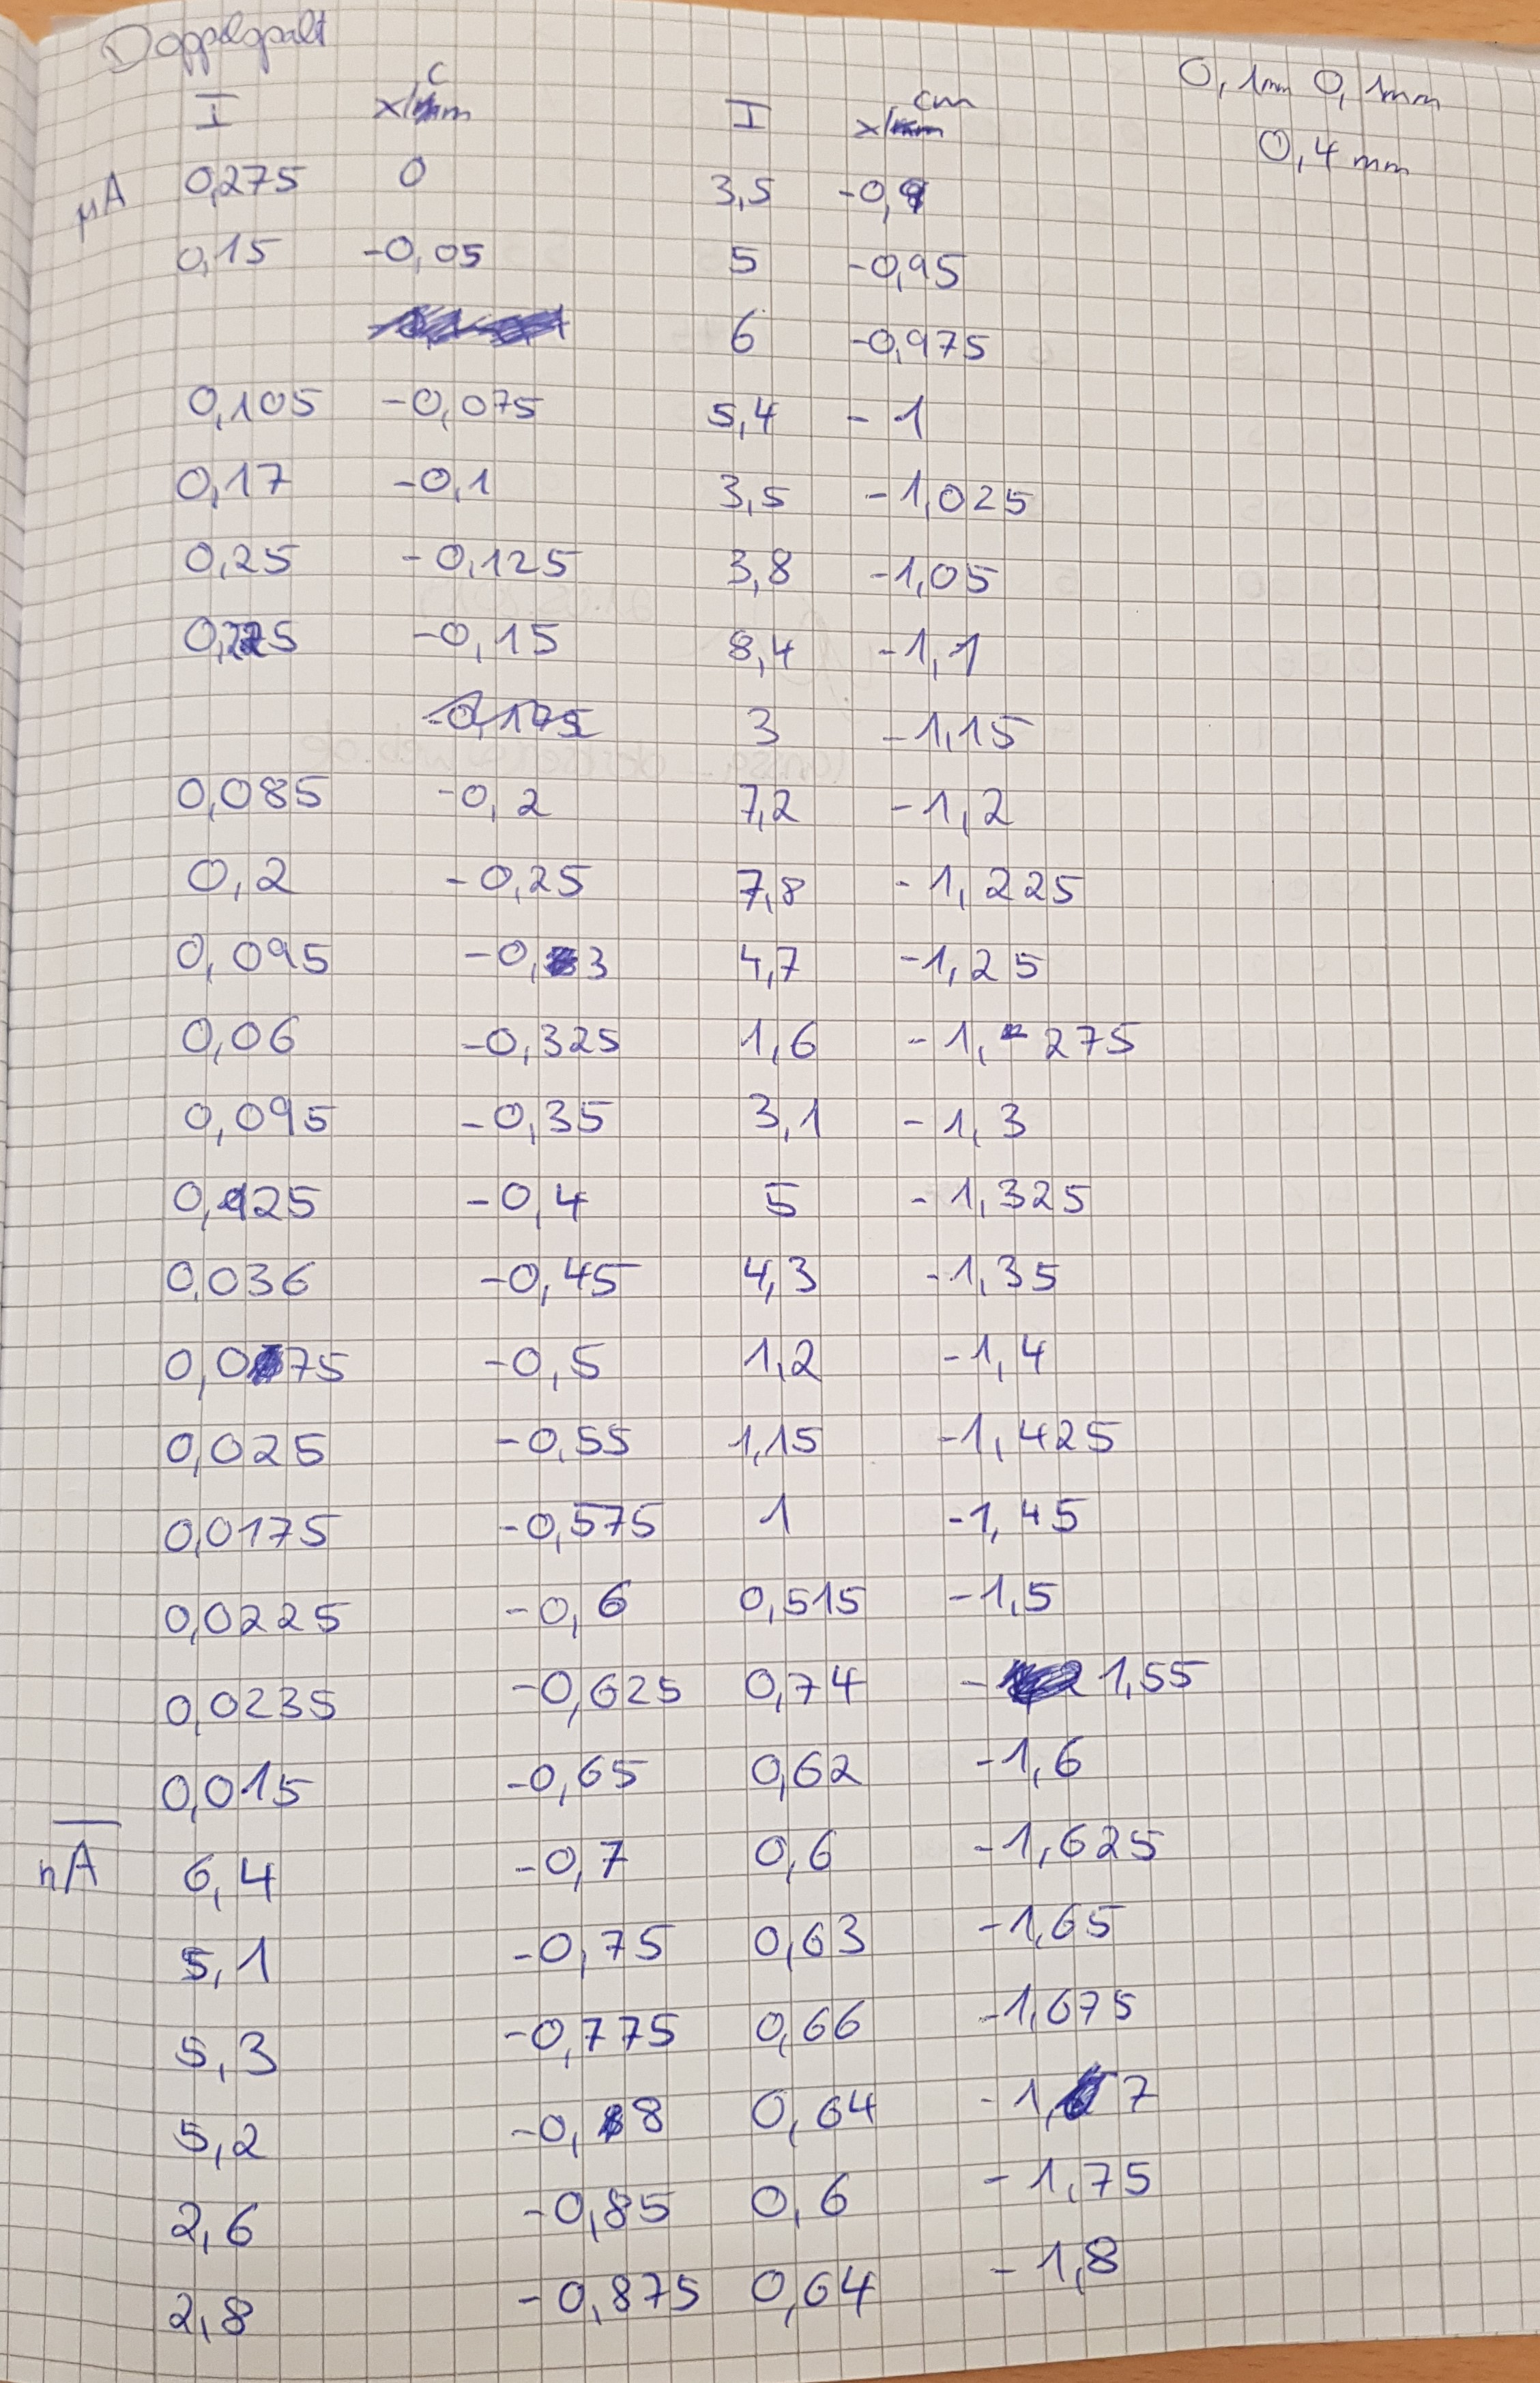
\includegraphics[height=24cm]{1 (5).jpg}
\end{figure}
\begin{figure}[H]
  \centering
  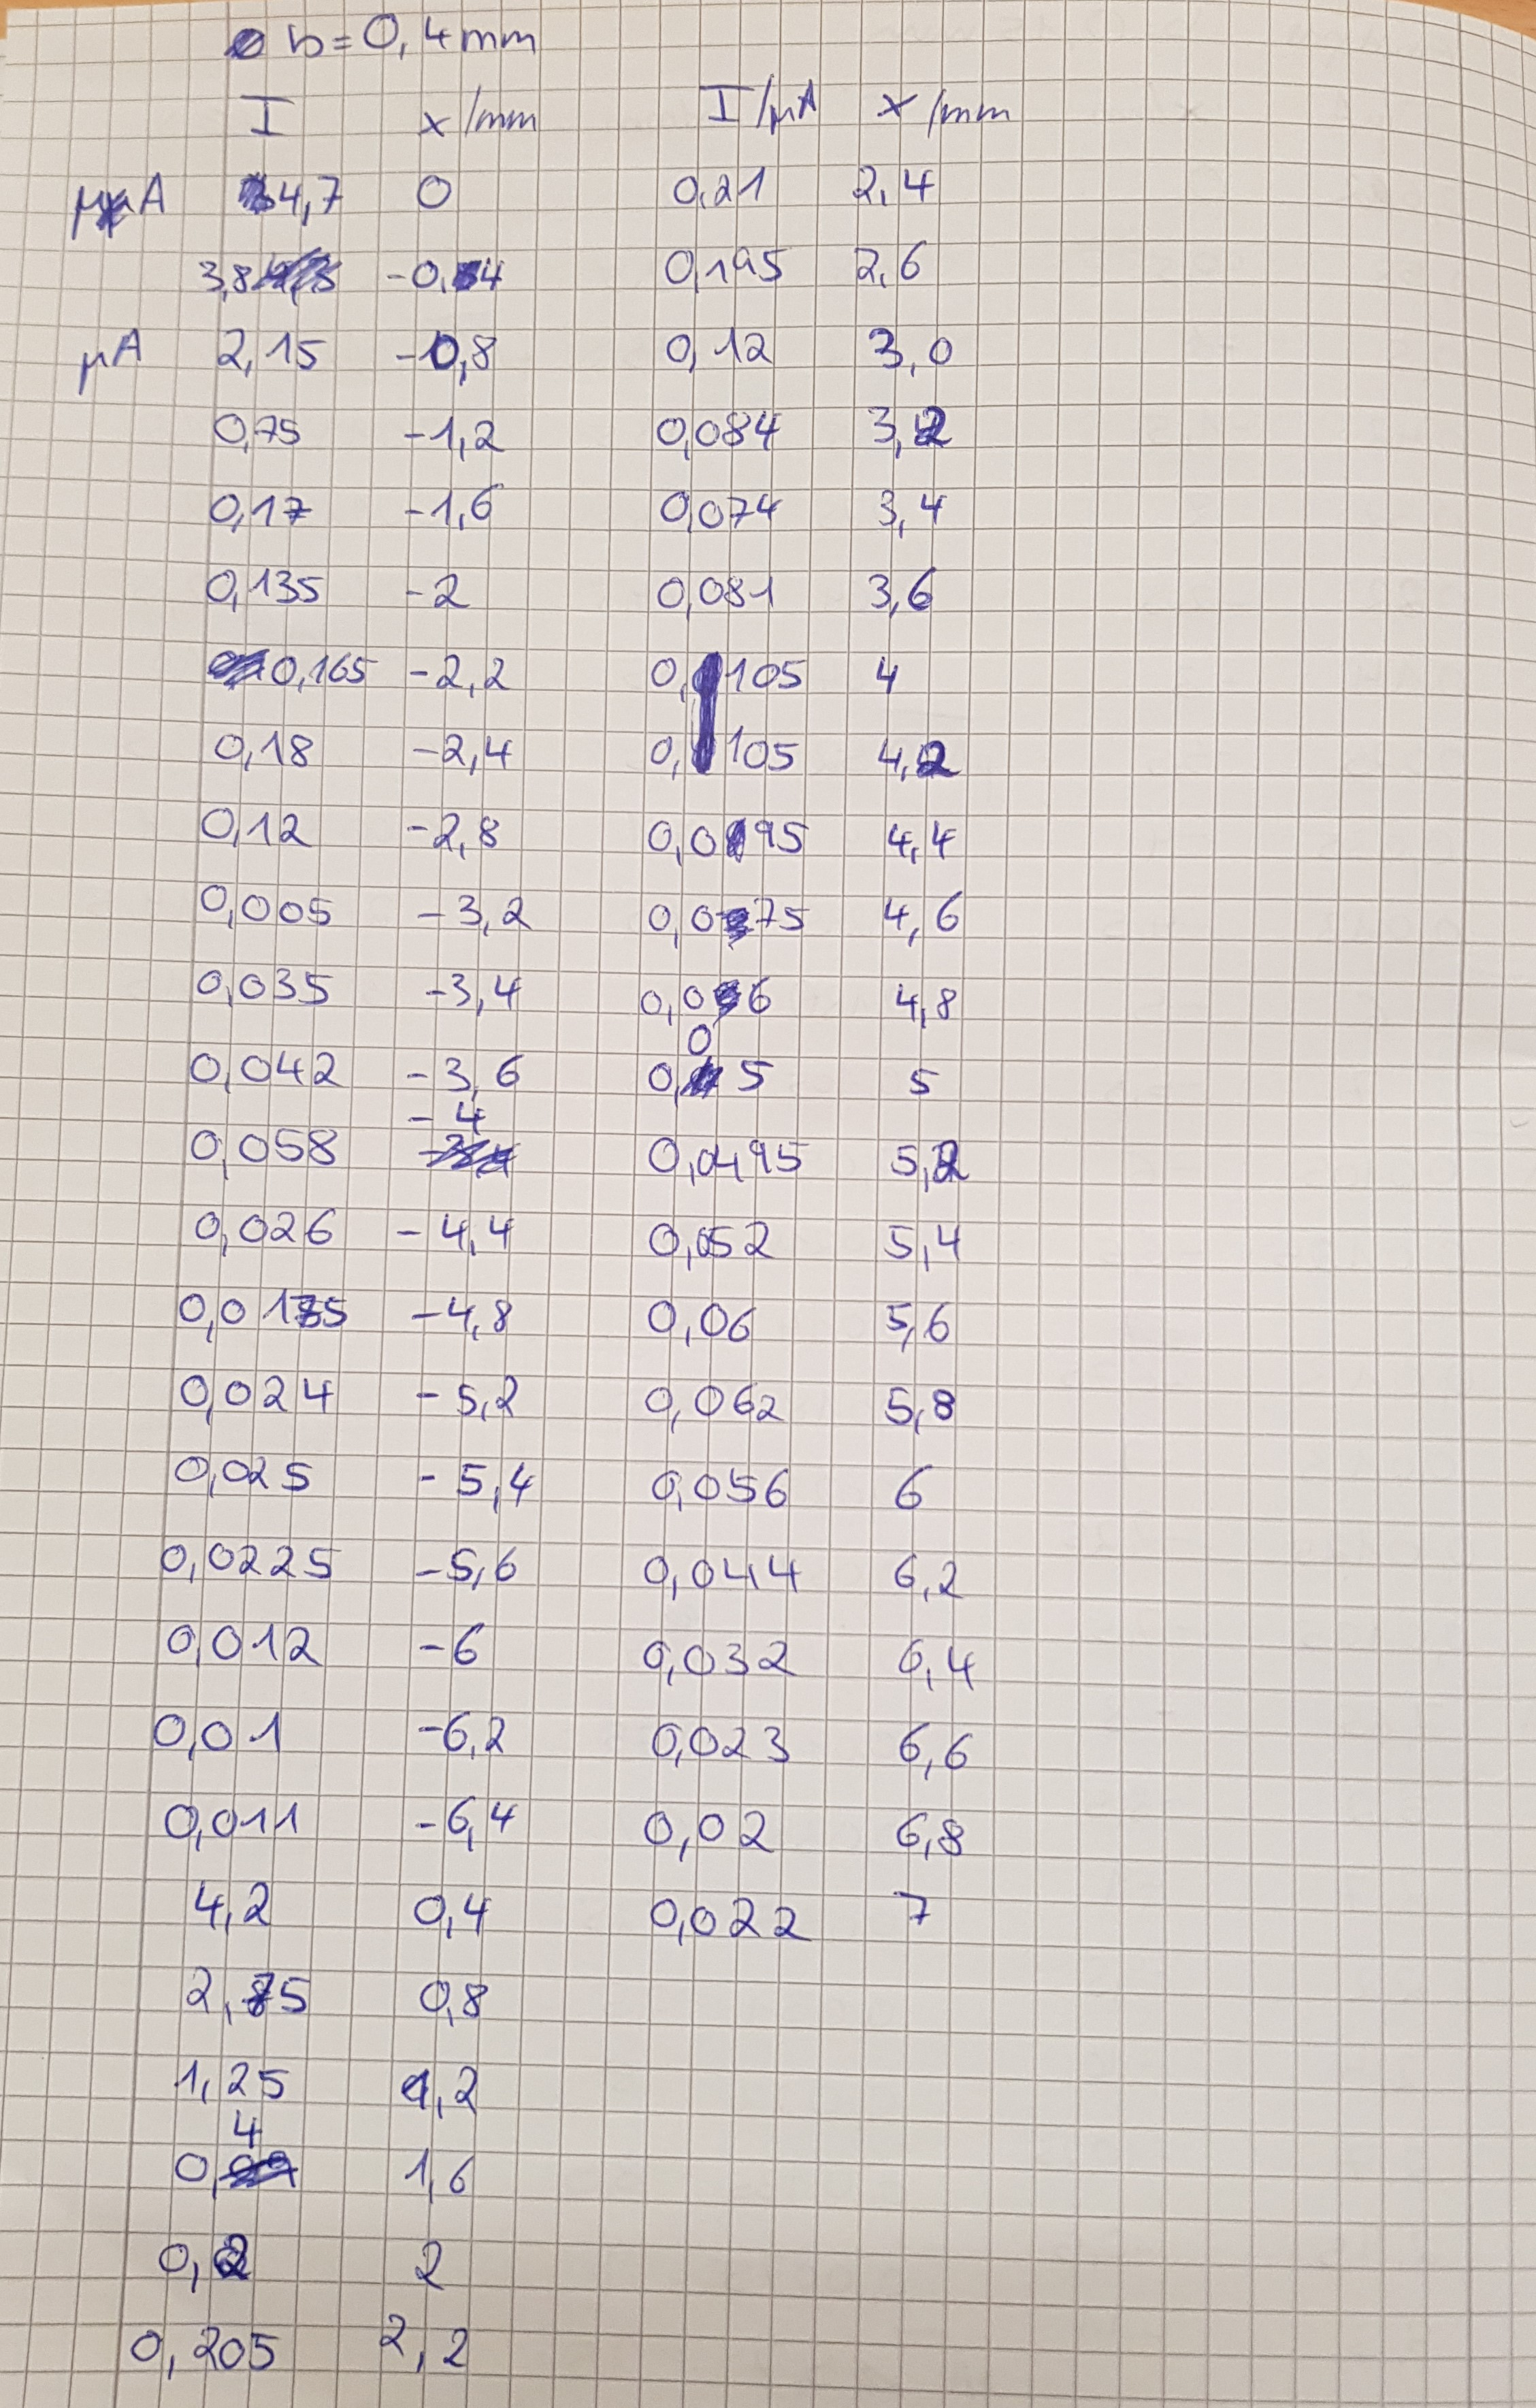
\includegraphics[height=24cm]{1 (4).jpg}
\end{figure}
\begin{figure}[H]
  \centering
  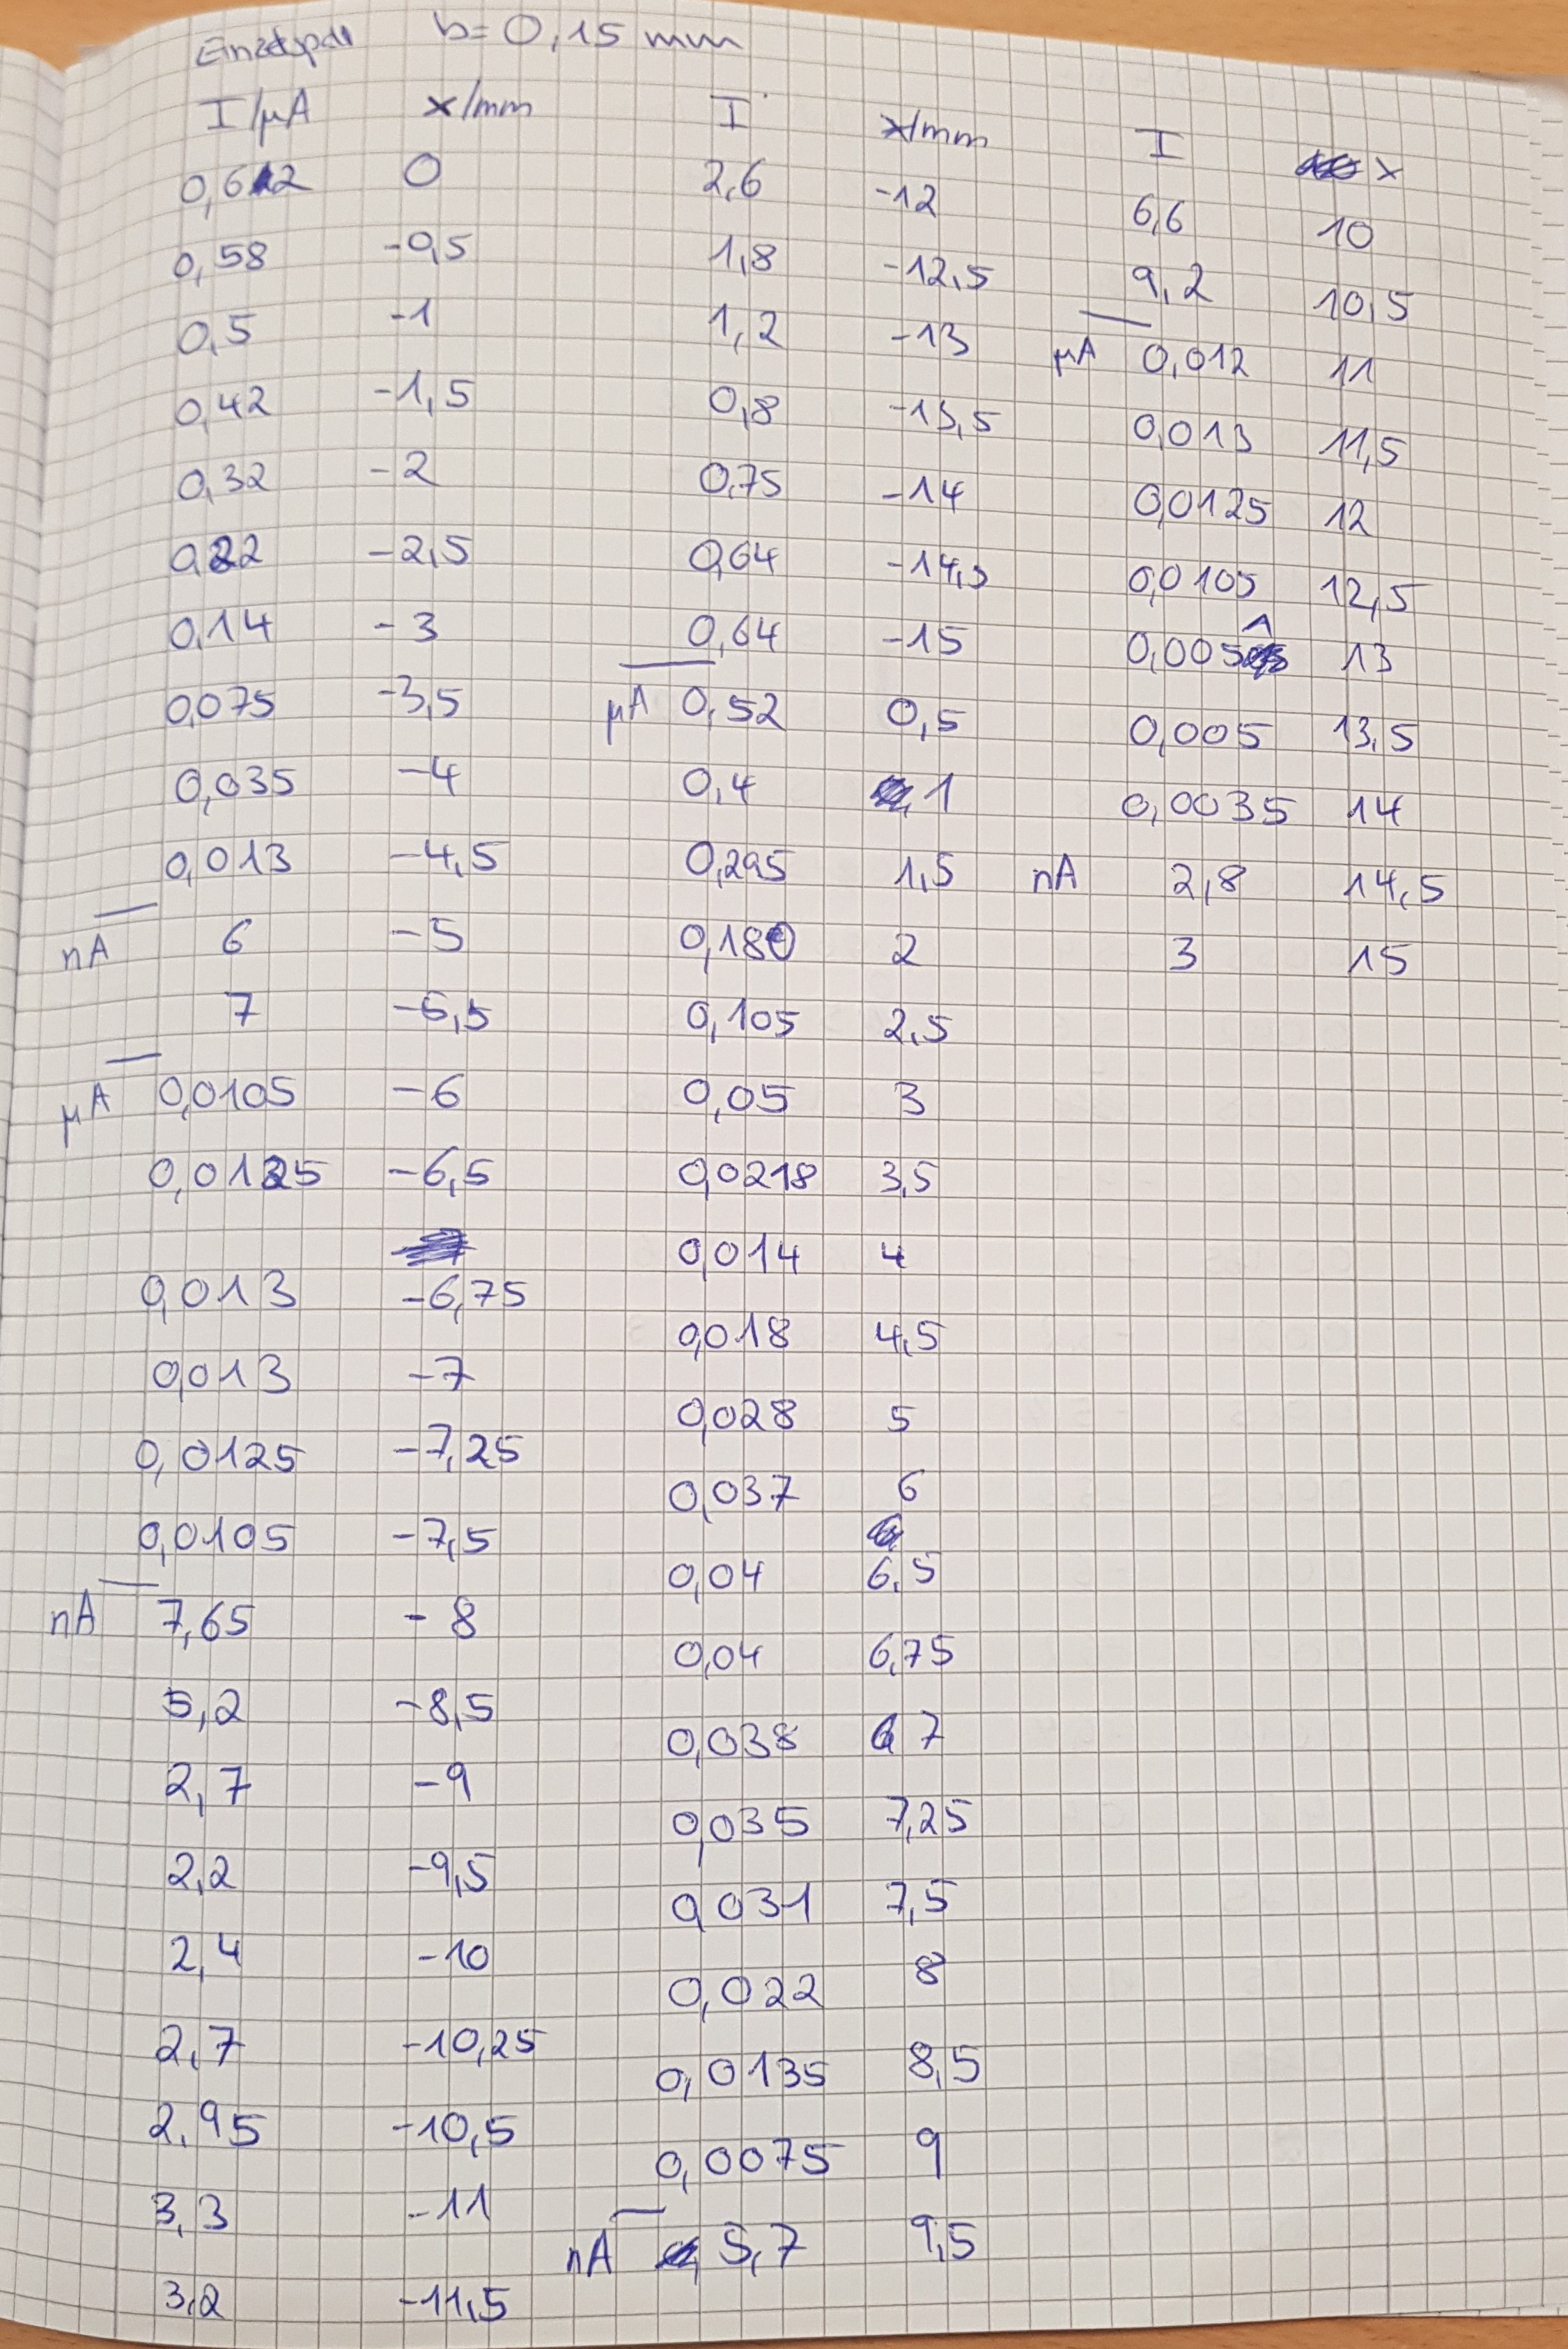
\includegraphics[height=24cm]{1 (3).jpg}
\end{figure}
\begin{figure}[H]
  \centering
  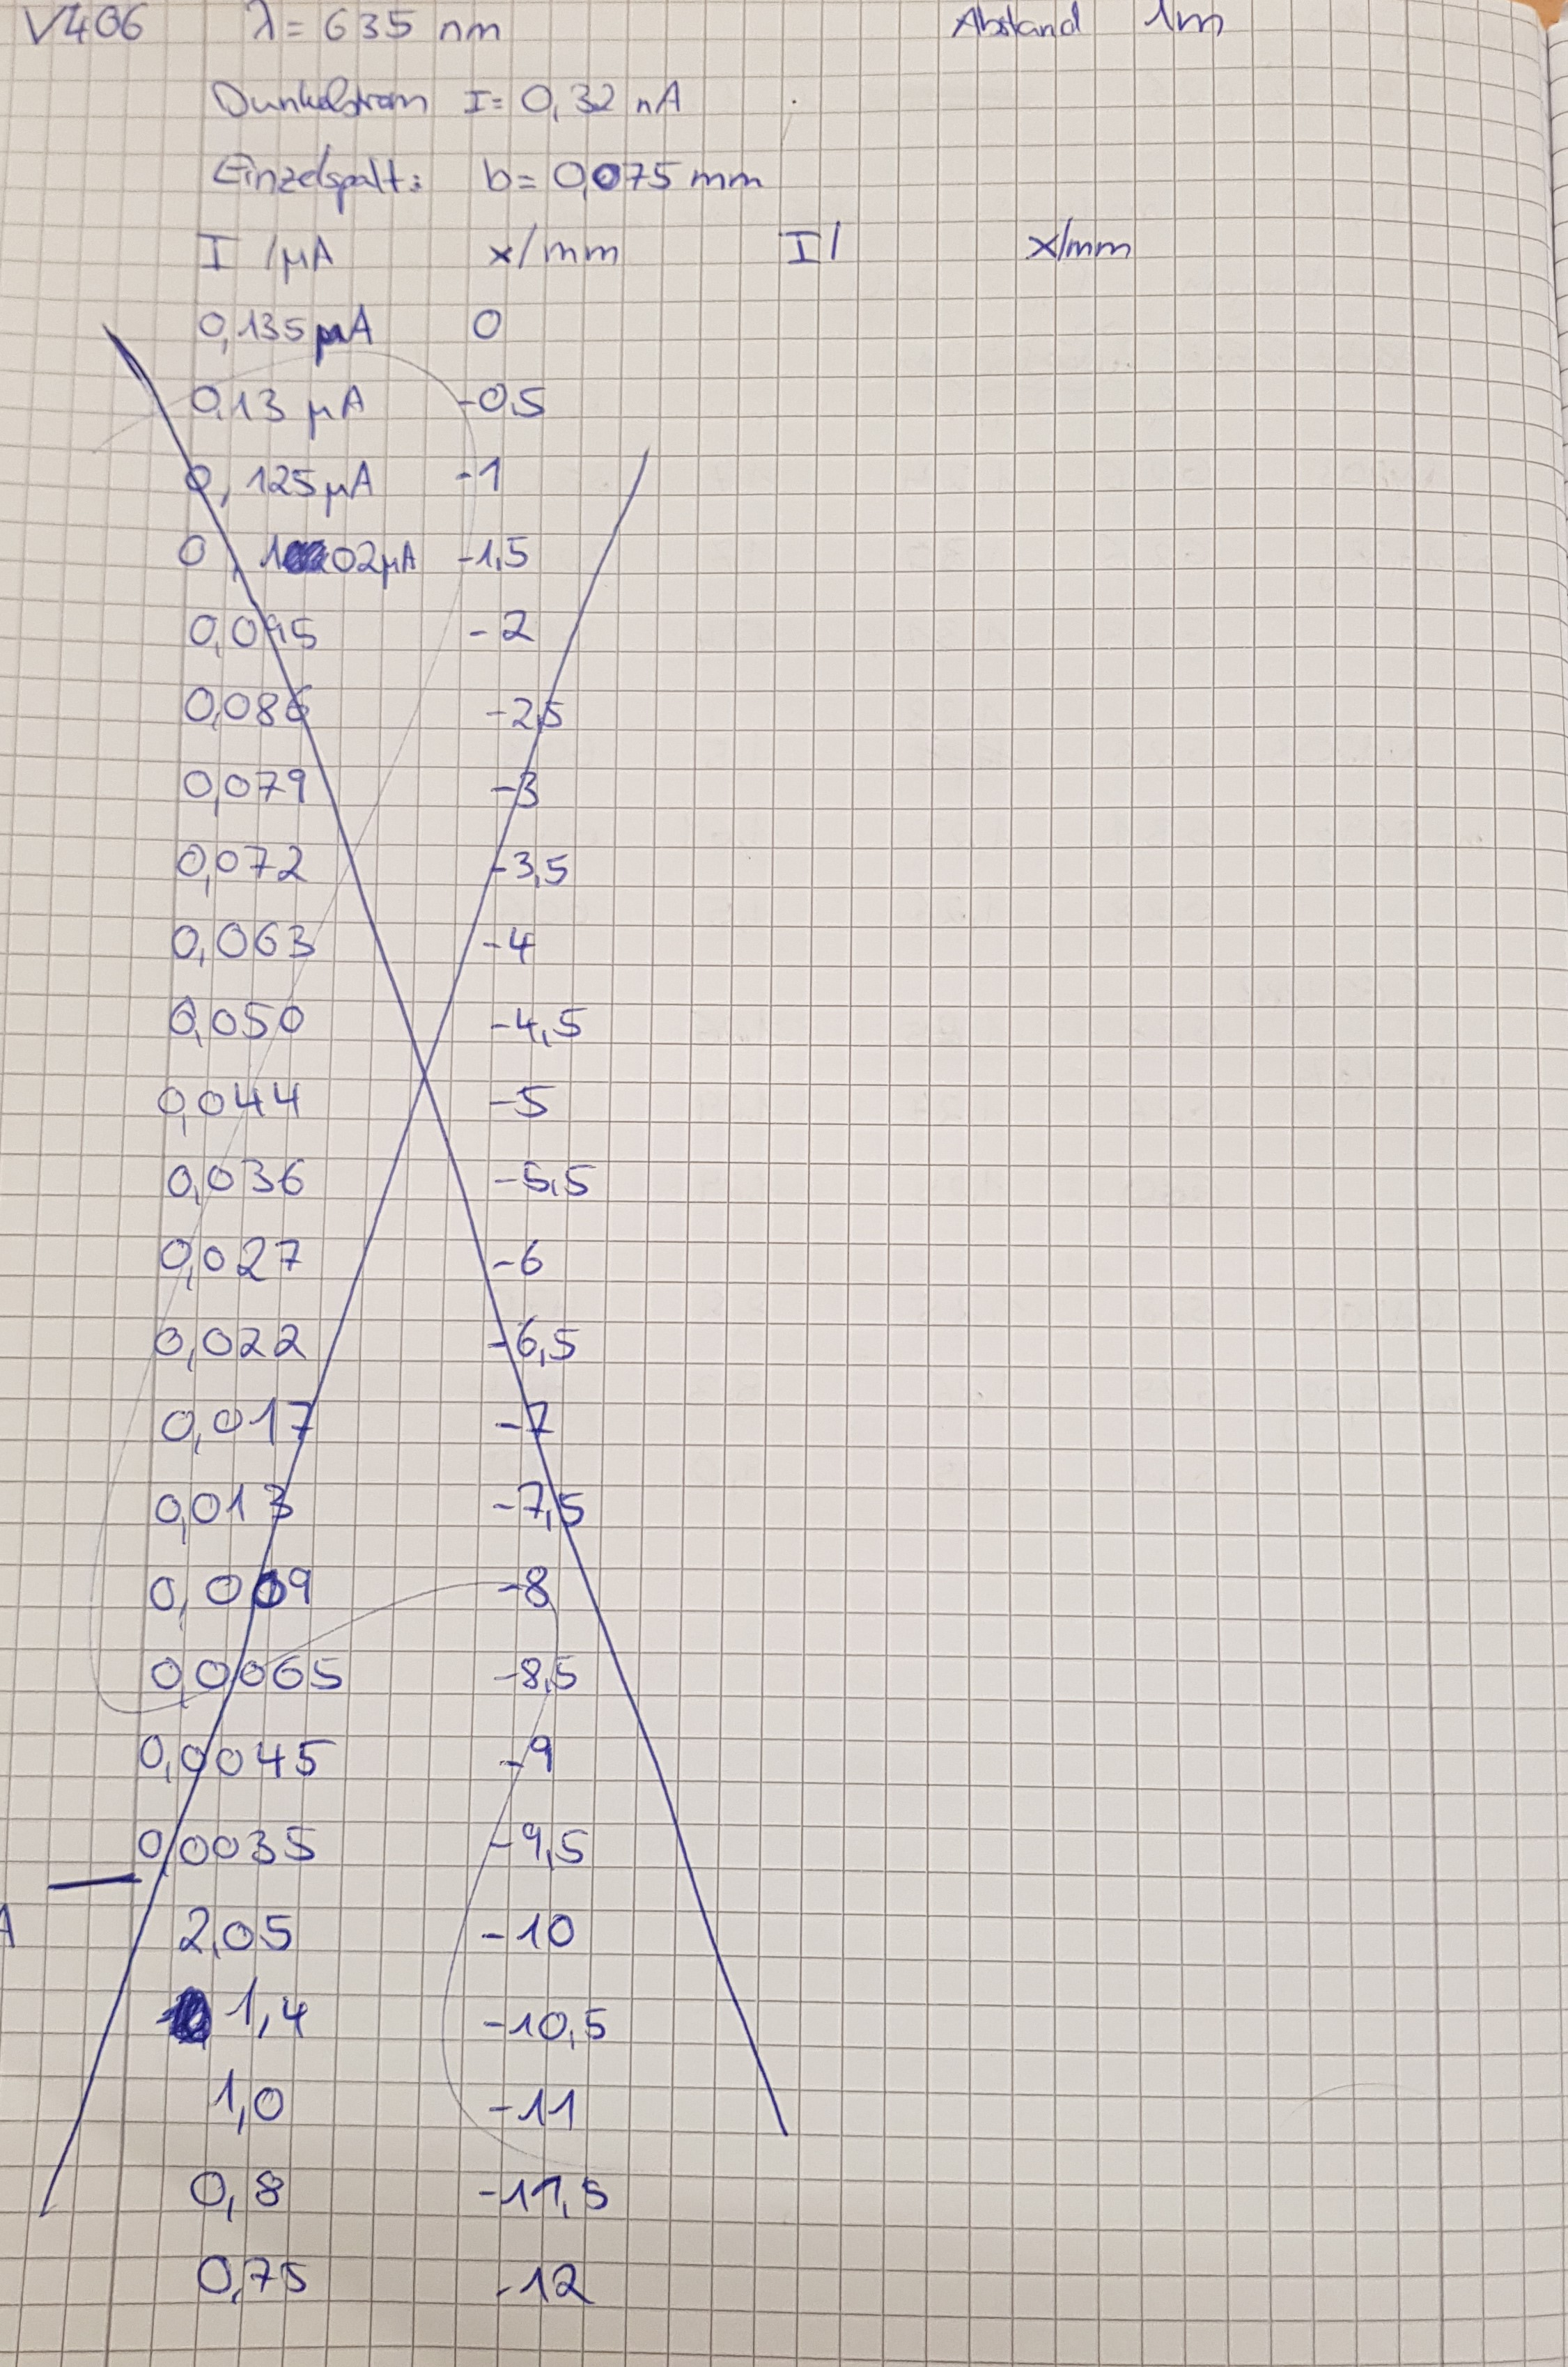
\includegraphics[height=24cm]{1 (2).jpg}
\end{figure}
\begin{figure}[H]
  \centering
  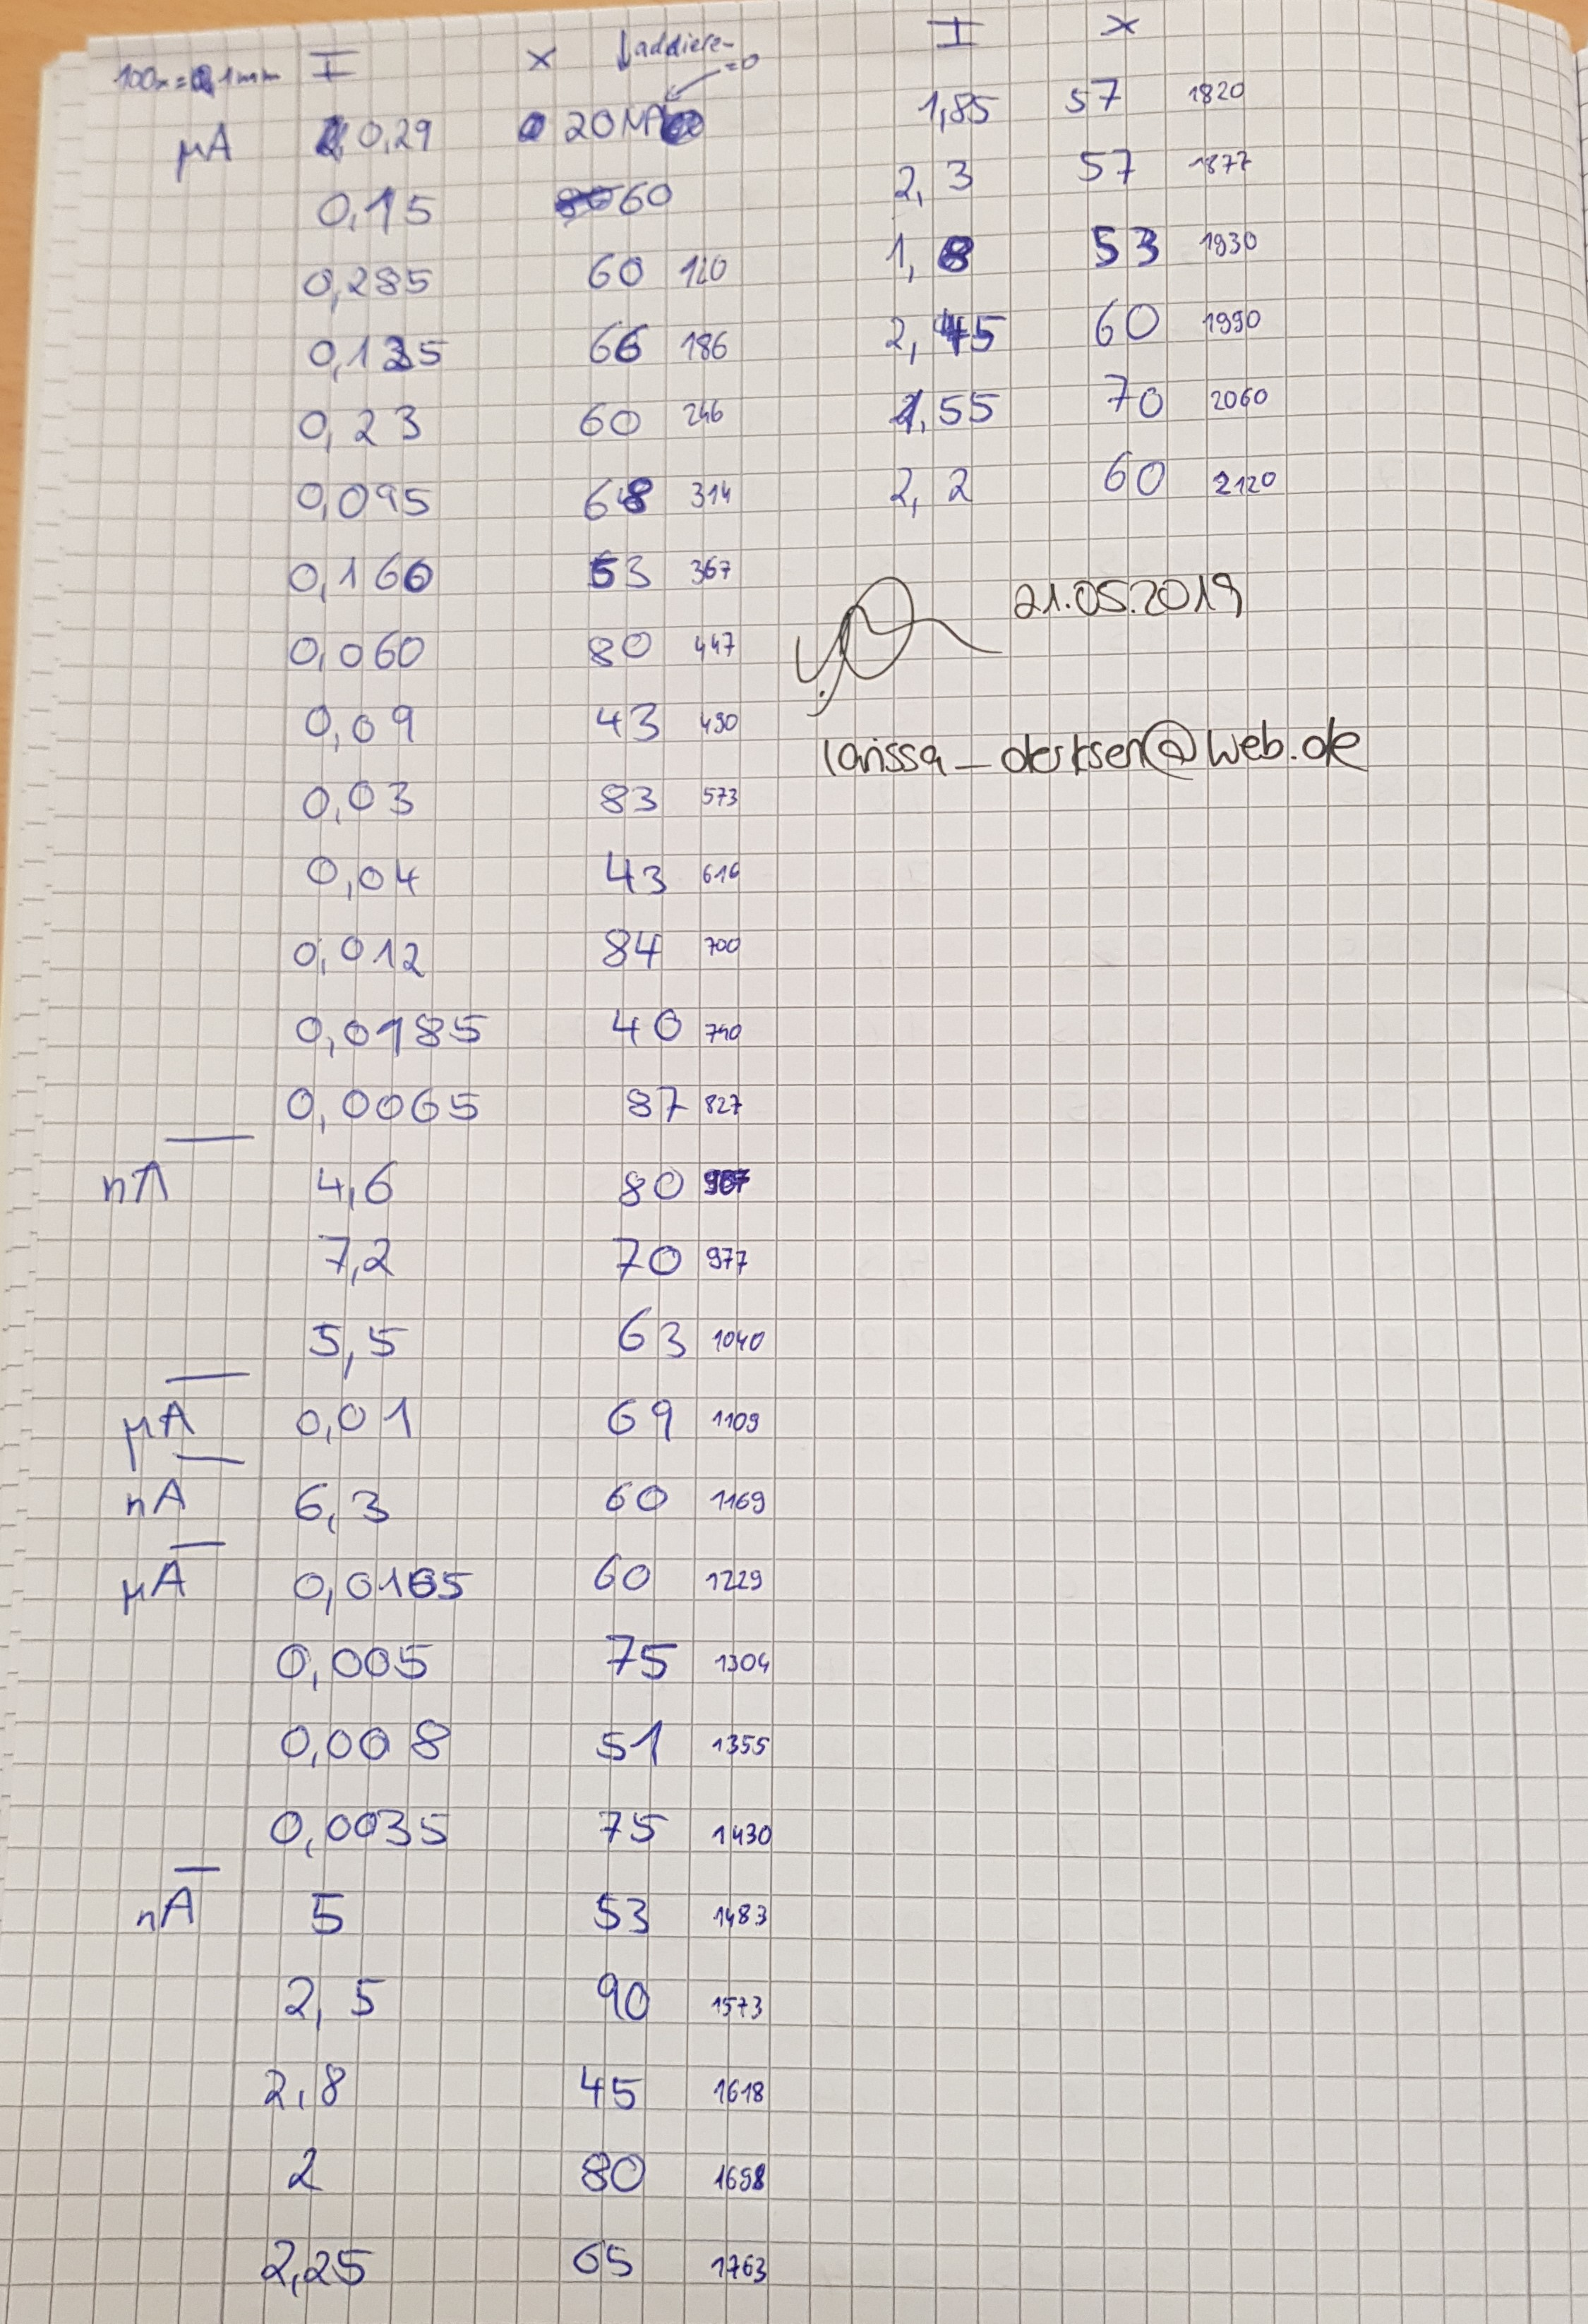
\includegraphics[height=24cm]{1 (1).jpg}
\end{figure}
